\section{Results}

\subsection{Multi-wavelength single-molecule co-localization (CoSMoS) methods}

Before describing the approach used for analysis of CoSMoS data, it is helpful to  review briefly the experimental method. The key features of a CoSMoS experiment include: 1) One species of fluorescently labeled molecule (called the “target”) is tethered to the surface of the observation chamber. Target molecules are immobilized at a surface density sufficiently low that the mean nearest-neighbor distance is large relative to the point-spread function (i.e., the diffraction-limited spot size) of the microscope.
2) Molecules, each species labeled with a different dye color, are added to the solution over the surface, typically at concentrations < 1 $\mu$M. When these “binder” molecules are freely diffusing in solution, they are invisible in TIRF. In contrast, when they are bound to the target, single binder molecules are detected as discrete fluorescent spots (Figure \ref{fig:cosmos_experiment}). The combination of features 1 and 2 means that formation of an individual binder-target complex is detected as spot appearance; dissociation of a binder-target complex is detected as spot disappearance \citep{Friedman2006-kb, Friedman2015-nx}.

CoSMoS data analysis requires identifying the locations of target molecules and the corresponding positions in the binder molecule camera channel. Image pre-processing steps include alignment of images from multiple wavelength channels and drift correction \citep{Friedman2015-nx, Smith2019-yb}. The CoSMoS data set consists of a set of images where we have $N$ target sites ($n \in \{1,\dots,N\}$) each consisting of a series of $F$ different images in a recording ($f \in \{1,\dots,F\}$) (a “recording”). Each image is a matrix (2D-array) of $P \times P$ pixel intensities ($i,j \in \{1,\dots,P\}$). We denote entire data set as a multi-dimensional array $D$ with the shape $N \times F \times P \times P$ where the value of a specific pixel intensity can be obtained by indexing as $D_{nfij}$. 

\begin{figure}
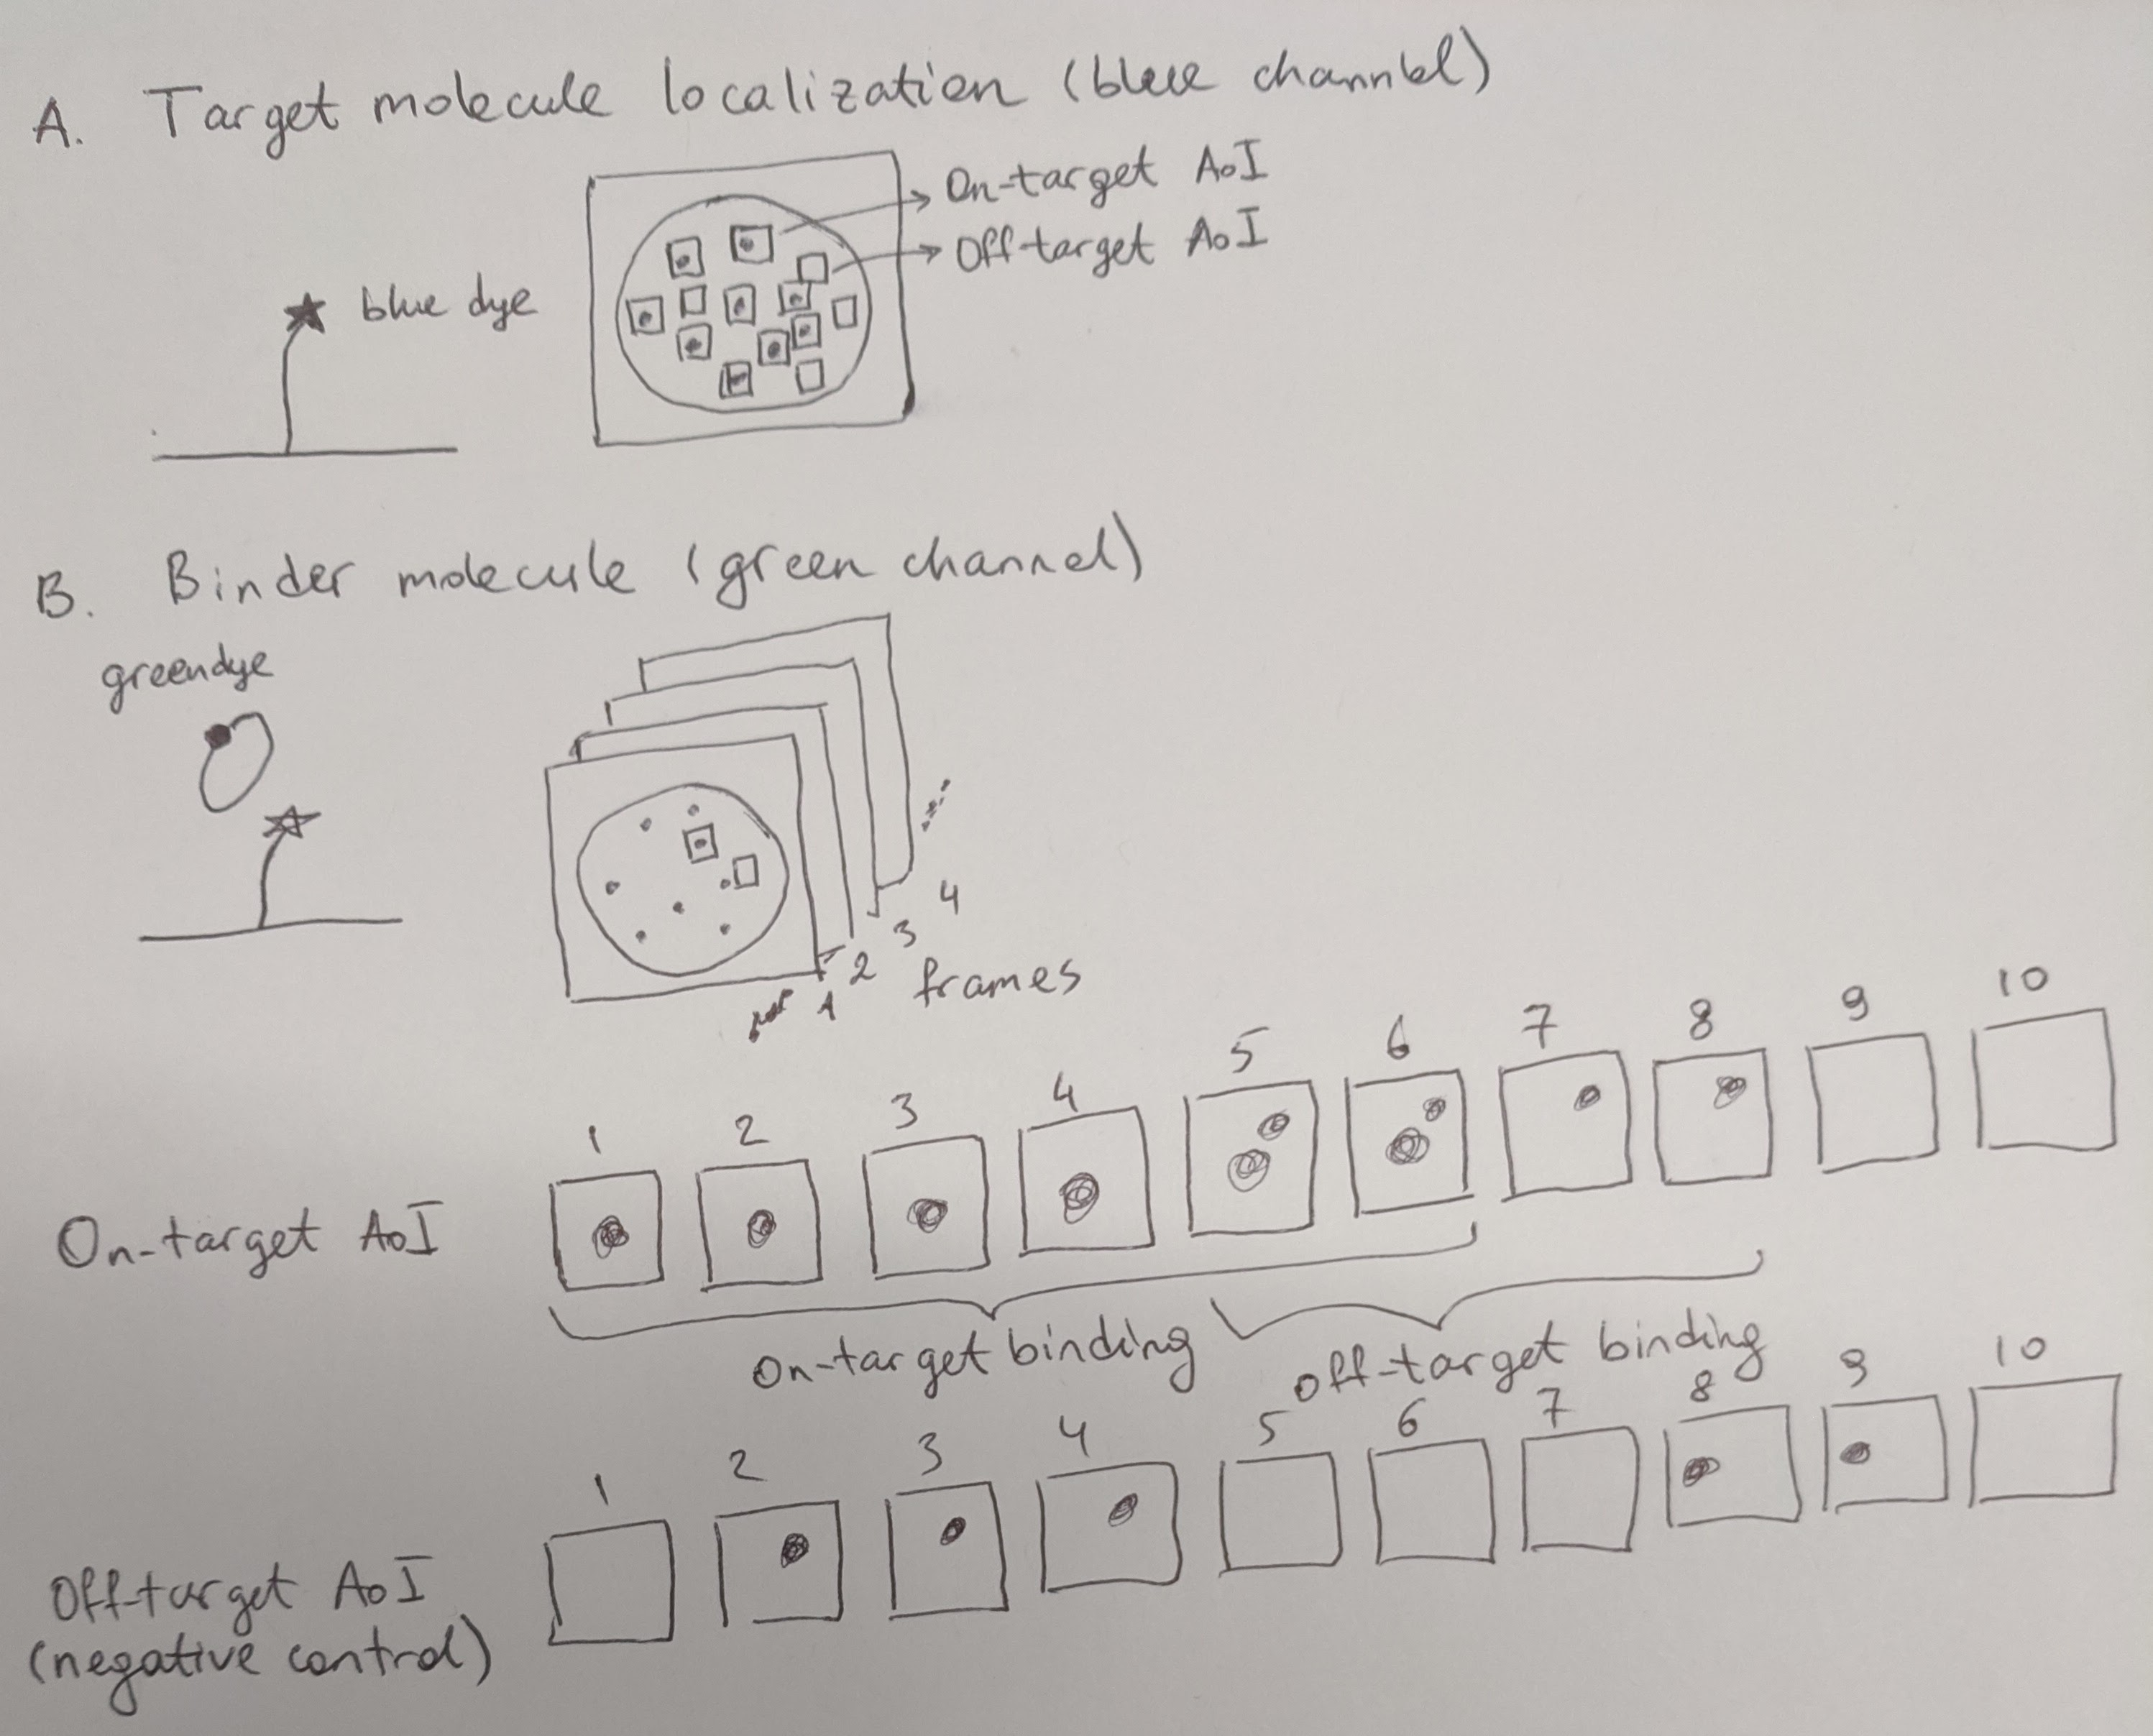
\includegraphics[width=\linewidth]{figures/figure1.jpg}
\caption{Co-localization single molecule spectroscopy experiment. (A) Target molecules are localized in the blue channel and then on-target and off-target areas of interest are selected. (B) Movies of the binder molecule collected in the green channel. In selected AoI binder molecules can be on-target, off-target, or absent.}
\label{fig:cosmos_experiment}
%% If the optional argument in the square brackets is "none", then the caption *will not appear in the main figure at all* and only the full caption will appear under the supplementary figure at the end of the manuscript.
%\figsupp[Shorter caption for main text.]{This is a supplementary figure's full caption, which will be used at the end of the manuscript.}{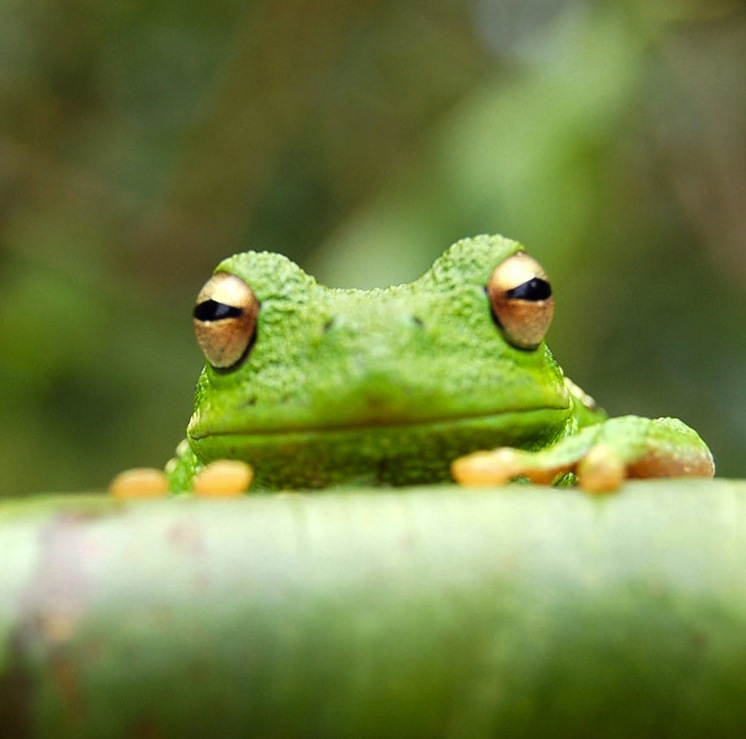
\includegraphics[width=6cm]{frog}}\label{figsupp:sf1}
%\figsupp{This is another supplementary figure.}{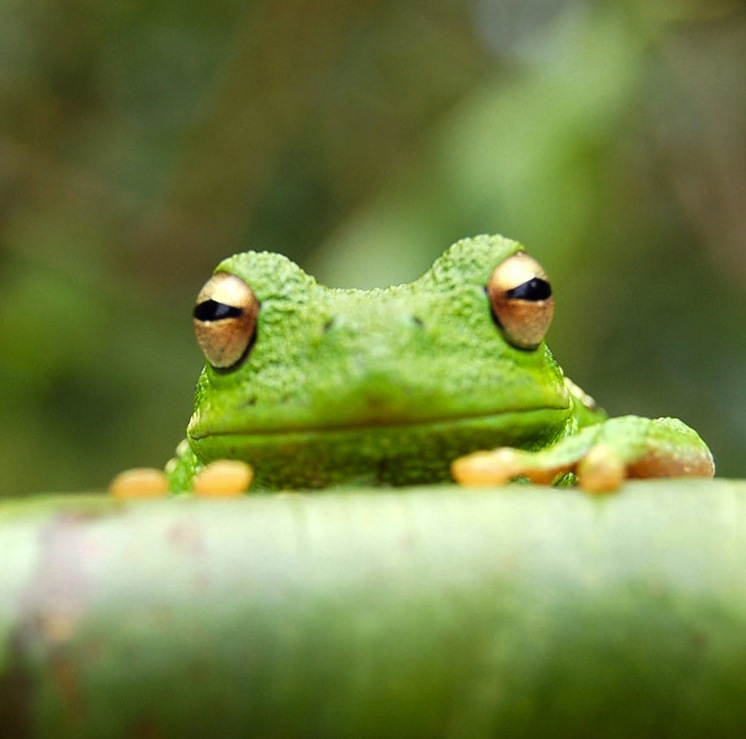
\includegraphics[width=6cm]{frog}}
%\figdata{This is a description of a data source.}\label{figdata:first}
%\figdata{This is another description of a data source.}\label{figdata:second}
\end{figure}

\subsection{Approach}

\subsubsection{Probabilistic modeling based on fundamental statistical analysis of data and priors}

To solve the problems with existing CoSMoS data analysis methods identified above, we have developed a new image-analysis-based approach that is accurate, objective, and built on a rigorous statistical approach to the CoSMoS image analysis problem. This method is based on probabilistic modeling methodology. Bayesian model is a statistical model where probability is used to represent all uncertainty within the model, both for observed and hidden quantities in a system of interest. Bayes' theorem allows to perform inference on hidden variables given the observed data. The method described here is time-independent meaning that we ignore the time dimension of the recording -- the order of the images is arbitrary and does not affect the model, as each image is considered statistically independent of the others. We note that this time-independent method can naturally be extended into a time-dependent approach to both more accurately analyze the images and to directly obtain information about molecular kinetic mechanisms.  The proposed methods will eliminate the need for subjective image inspection and minimize the manual work required for CoSMoS data analysis.

\subsubsection{Image model}

Distinctive feature of our approach is that we directly model 2D images at target sites which has not been previously done to our knowledge. CoSMoS images consist of background intensity and diffraction-limited spots. Local background intensity of the image is parameterized by a scalar $b_{nf}$. Fluorescence spot is modeled as a 2D Gaussian which accurately approximates fluorescence microscope point spread function \citep{Zhang2007-rb}. Our model assumes that at maximum $K$ number of spots can be present in a single image. Each individual spot ($k \in \{1,\dots,K\}$) is parameterized by binary spot existence variable ($m_{knf} \in \{0,1\}$), integrated spot intensity ($h_{knf}$), spot width ($w_{knf}$), and position of the spot relative to the target ($x_{knf},y_{knf}$). When the spot is absent ($m_{knf}=0$) the intensity is zero or at the baseline level. The ideal shape of the image ($\mu^D_{nf}$) is calculated as the sum of the background intensity and 2D Gaussian spots present in the image (see Methods). Figure \ref{fig:model} shows ideal image shapes for cases when there are no spots (A), one spot (B), and two spots (C). Finally, each image has an index variable for the on-target spot ($\theta_{nf} \in \{0,1,\dots,K\}$) where zero means that the on-target spot is absent.

\subsubsection{Noise model}

Scatter about the expected value of pixel intensity ($\mu^D_{nfij}$) is determined by photonic shot noise and the gain of the camera. Shot noise originates from a stochastic nature of photon counting which can be modeled by a Poisson process. The number of photons that fall on each pixel of the camera is Poisson distributed where the variance of the signal equals the mean value of the signal. Gain is a camera setting that amplifies the signal from camera sensors. Our model uses Gamma distribution parameterized by mean intensity ($\mu^D_{nfij}$) and gain ($g$) to model the linear relationship between the expected value of the signal and the variance with which the signal scatter about its expected value. Figure \ref{fig:model}  shows images  where the ideal images were perturbed with Gamma noise for no-spot (D), single spot (E), and two spots (F) images.

\subsubsection{Spot detection}

Current spot detection methods produce binary outputs by using a bandpass-filter set by a user-specified intensity threshold \citep{Friedman2015-nx, Smith2019-yb}. To analyze the spot detection problem within the Bayesian framework we model spot intensities ($h_{knf}$) as a mixture of distribution of two classes with the hidden variable $m_{knf}$ specifying the identity of the class: a) no-spot baseline intensity distribution when $m_{knf}=0$ and b) spot intensity distribution of a binder molecule when $m_{knf}=1$. Unlike previous methods, this approach discriminates authentic fluorescence spots from fluctuations in background fluorescence in a probabilistic manner and assigns probabilities of belonging to each class.

\subsubsection{Co-localization detection}

We employ the similar approach to detect co-localization events and model the center of the spot to be distributed according to a mixture of two distributions (Figure \ref{fig:model}G). We model non-specific binding events explicitly with a uniform distribution of the center of the spot since non-specific binding can occur anywhere within the image. On the other hand, co-localized spot denoted by an index variable $\theta_{nf}$ is scattered around target location within the co-localization accuracy which is modeled by distribution centered on target with the standard deviation equal to the co-localization accuracy. Again, co-localization detection is performed in a probabilistic manner and for each spot probabilities of being on-target and off-target are calculated. It is important to note that spot detection and co-localization detection are part of a single unified model, rather than separate steps of the analysis.

\begin{figure}
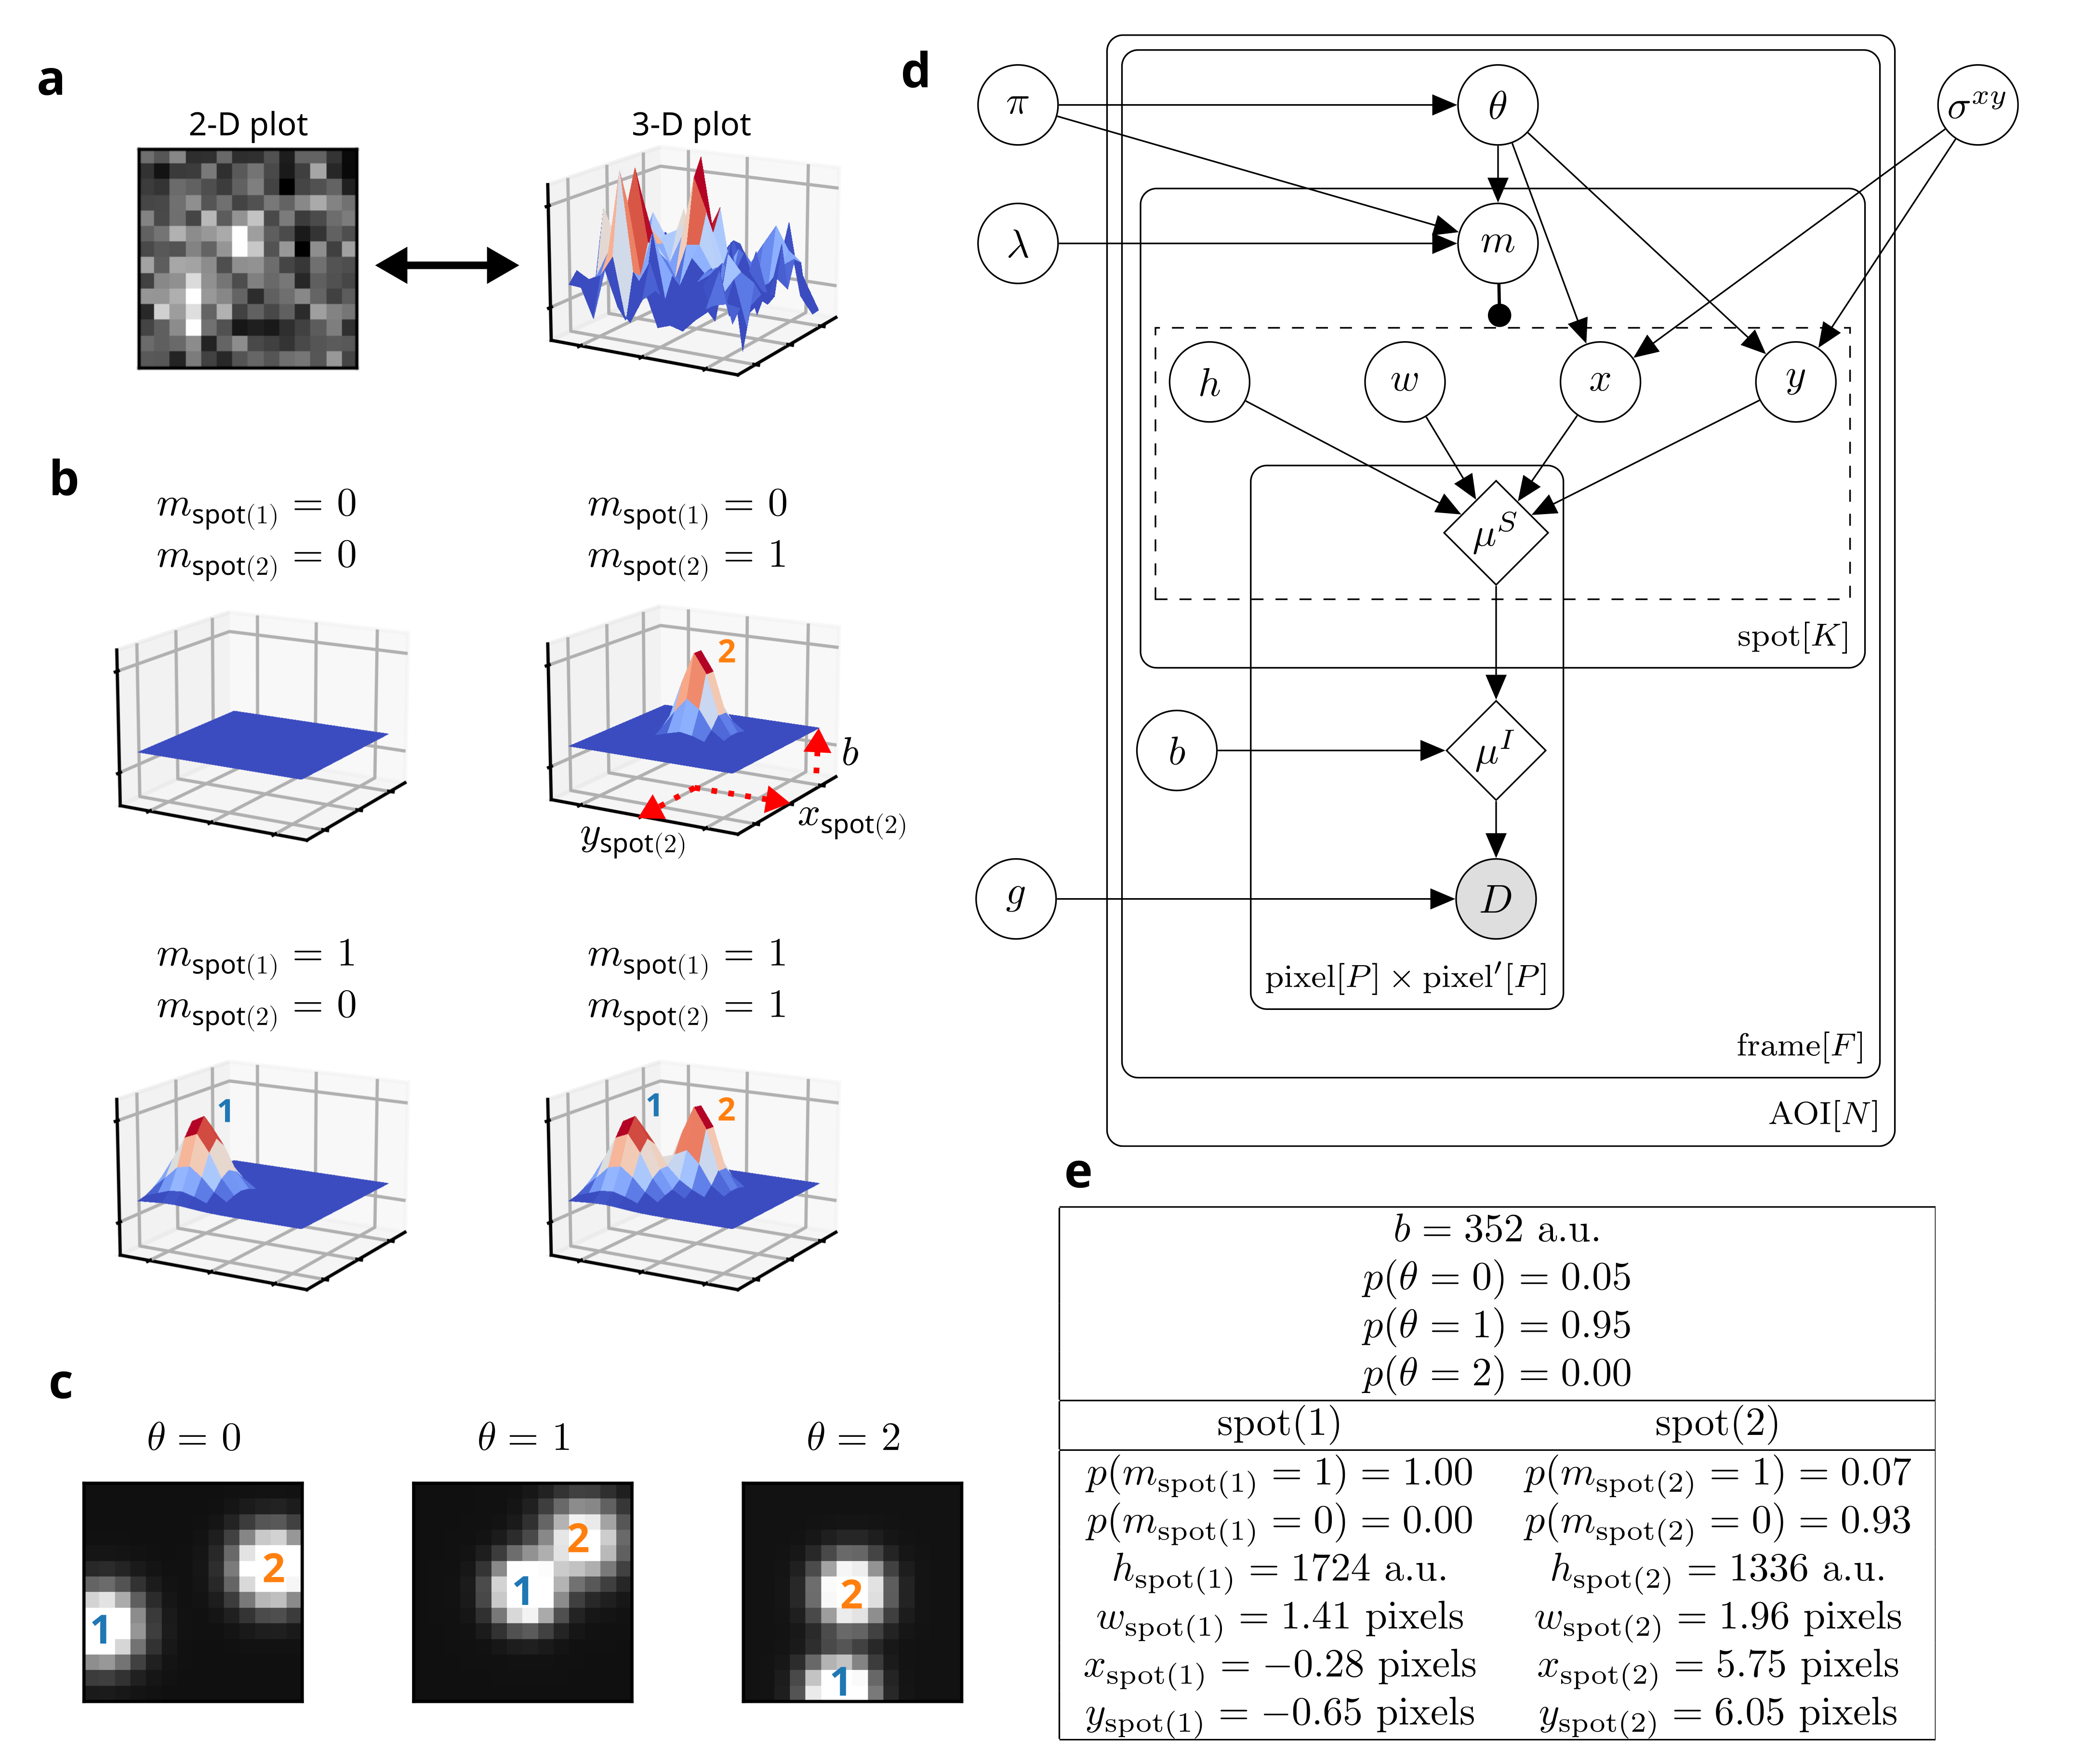
\includegraphics[width=\linewidth]{figures/figure2/figure2.png}
%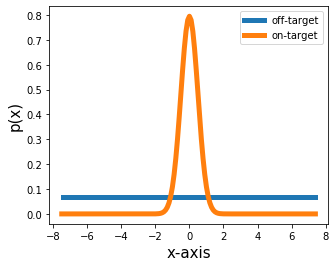
\includegraphics[width=\linewidth]{figures/figure2g.png}
\caption{Image models. CoSMoS images are modeled as 2D Gaussian spots superimposed onto the background intensity. Examples of the ideal image shapes for cases when there are (A) no spots, (B) single on-target spot, (C) single off-target spot, and (D) two spots. Noisy images (E-H) are generated using Gamma distribution with the parameter gain = 7 as described in the text.}
\label{fig:model}
\end{figure}

\begin{figure}
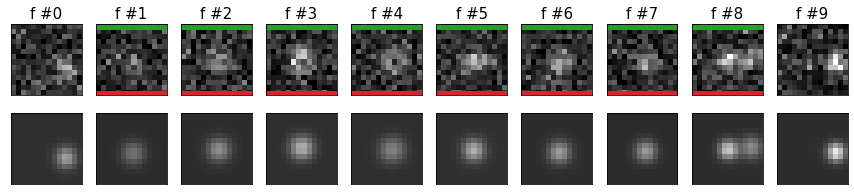
\includegraphics[width=\linewidth]{figures/figure3a.png}
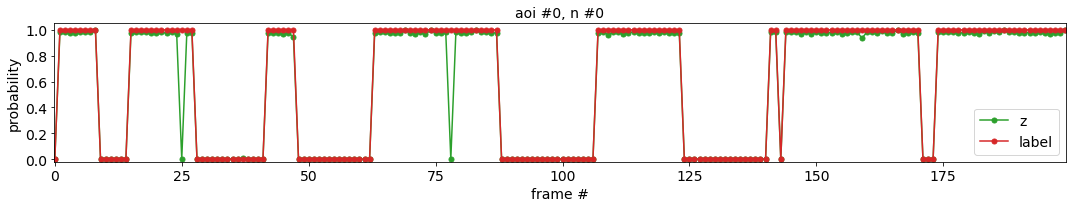
\includegraphics[width=\linewidth]{figures/figure3b.png}
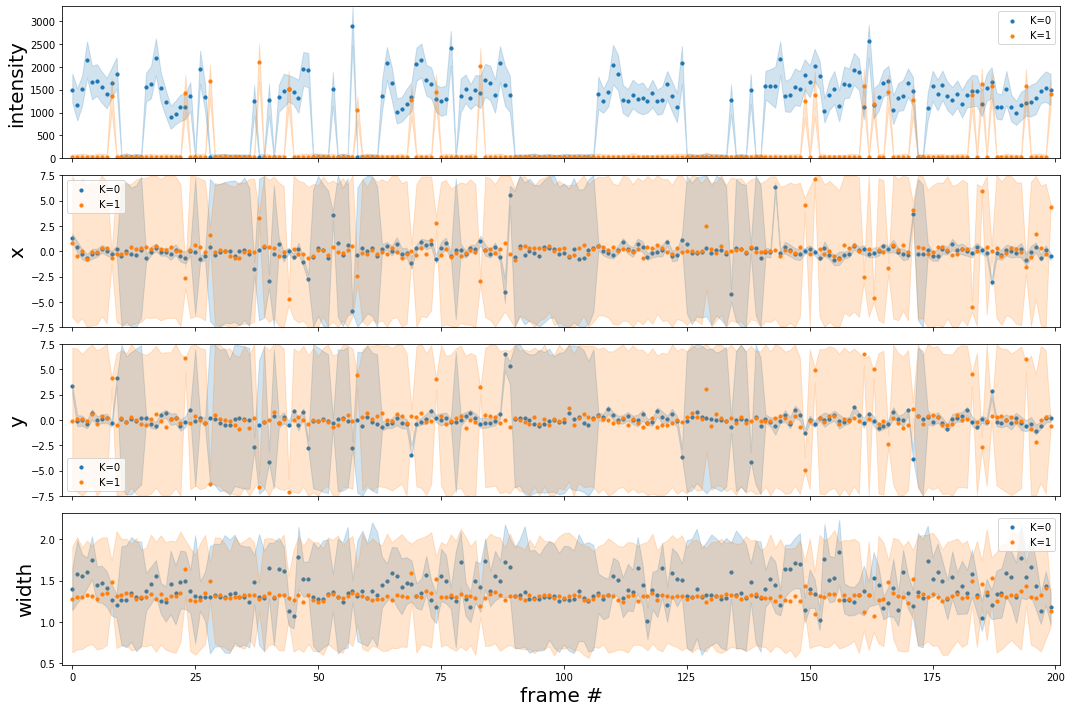
\includegraphics[width=\linewidth]{figures/figure3c.png}
\caption{Co-localization single molecule spectroscopy experiment. (A) Target molecules are localized in the blue channel and then on-target and off-target areas of interest are selected. (B) Movies of the binder molecule collected in the green channel. In selected AoI binder molecules can be on-target, off-target, or absent.}
\label{fig:view}
\end{figure}

\subsection{Comparison of Bayesian method with heuristic spot thresholding}

We have done two types of performance comparison between the Bayesian method and the heuristic spot thresholding method.

\subsubsection{Experimental data}

For the first performance comparison, images from real (i.e., not simulated) experimental data recordings were analyzed. In this experiment, we labeled the NusG protein with an orange dye. We then tethered to a microscope slide blue-dye-labeled DNA molecules at very low surface density (so that each molecule is resolved as a separate fluorescent spot) and observed real-time binding and dissociation of the other labeled molecules during the transcription process and its regulation. The signal from the orange dye was split between short wavelength and long wavelength channels. The signal in the short wavelength channel was attenuated to varying degree to produce data sets with a range of SNR. Images from the long wavelength channel with high SNR were analyzed to determine "true" identities of the images.

Each data set was analyzed by both the Bayesian method and the heuristic spot thresholding algorithm (Figure \ref{fig:real_data}). By comparison with the known “true” identities of the images, the accuracy of the resulting classifications was judged using a variety of specialized statistics for binary classification data, including true and false positive rates, true and false negative rates, and the Matthews Correlation Coefficient (MCC) \citep{Fawcett2006-bq, Matthews1975-rw}. The MCC statistic is widely regarded as a single overall, balanced measure which is meaningful even when the classes are of very different sizes. The MCC corresponds to the Pearson correlation coefficient between the estimated and “true” binary classifications. MCC=+1 represents a perfect prediction, MCC=0 a perfectly random prediction, and MCC=-1 indicates maximal disagreement between truth and estimation. Over a range of S/N, the Bayesian method gave image classification accuracy (as quantified by the MCC) better than the heuristic spot thresholding algorithm. 

\begin{figure}
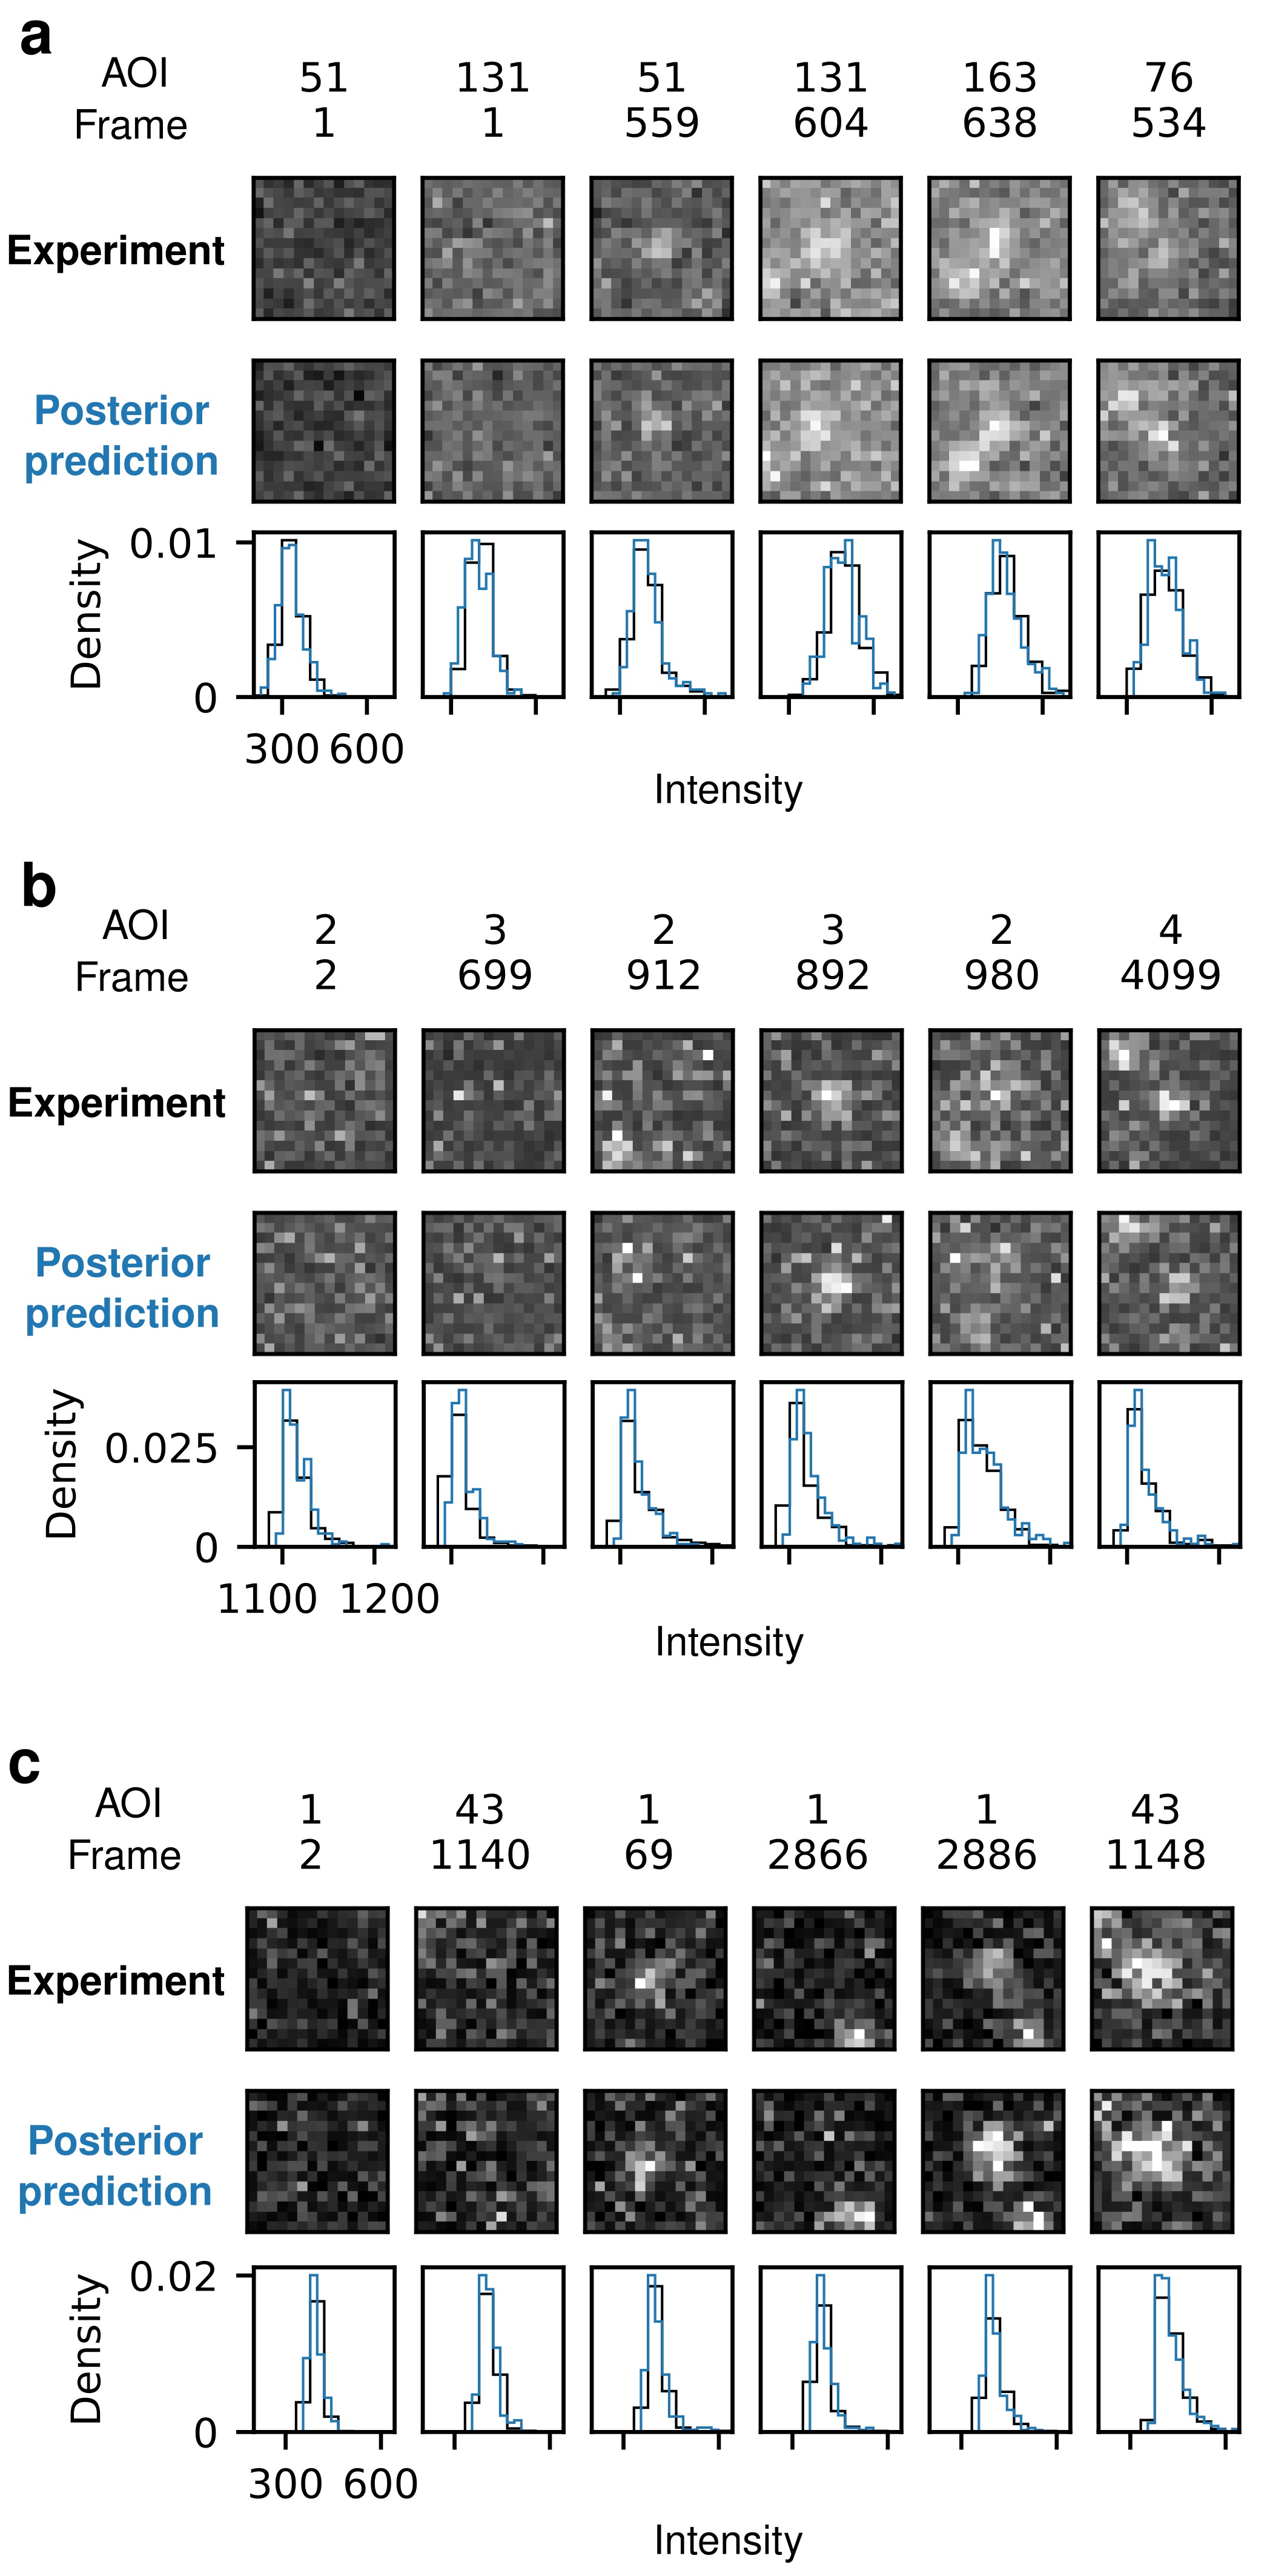
\includegraphics[width=\linewidth]{figures/figure4/figure4.png}
\caption{Performance comparison of the Bayesian method with the heuristic spot thresholding algorithm on real experimental data.}
\label{fig:real_data}
\end{figure}

\begin{figure}
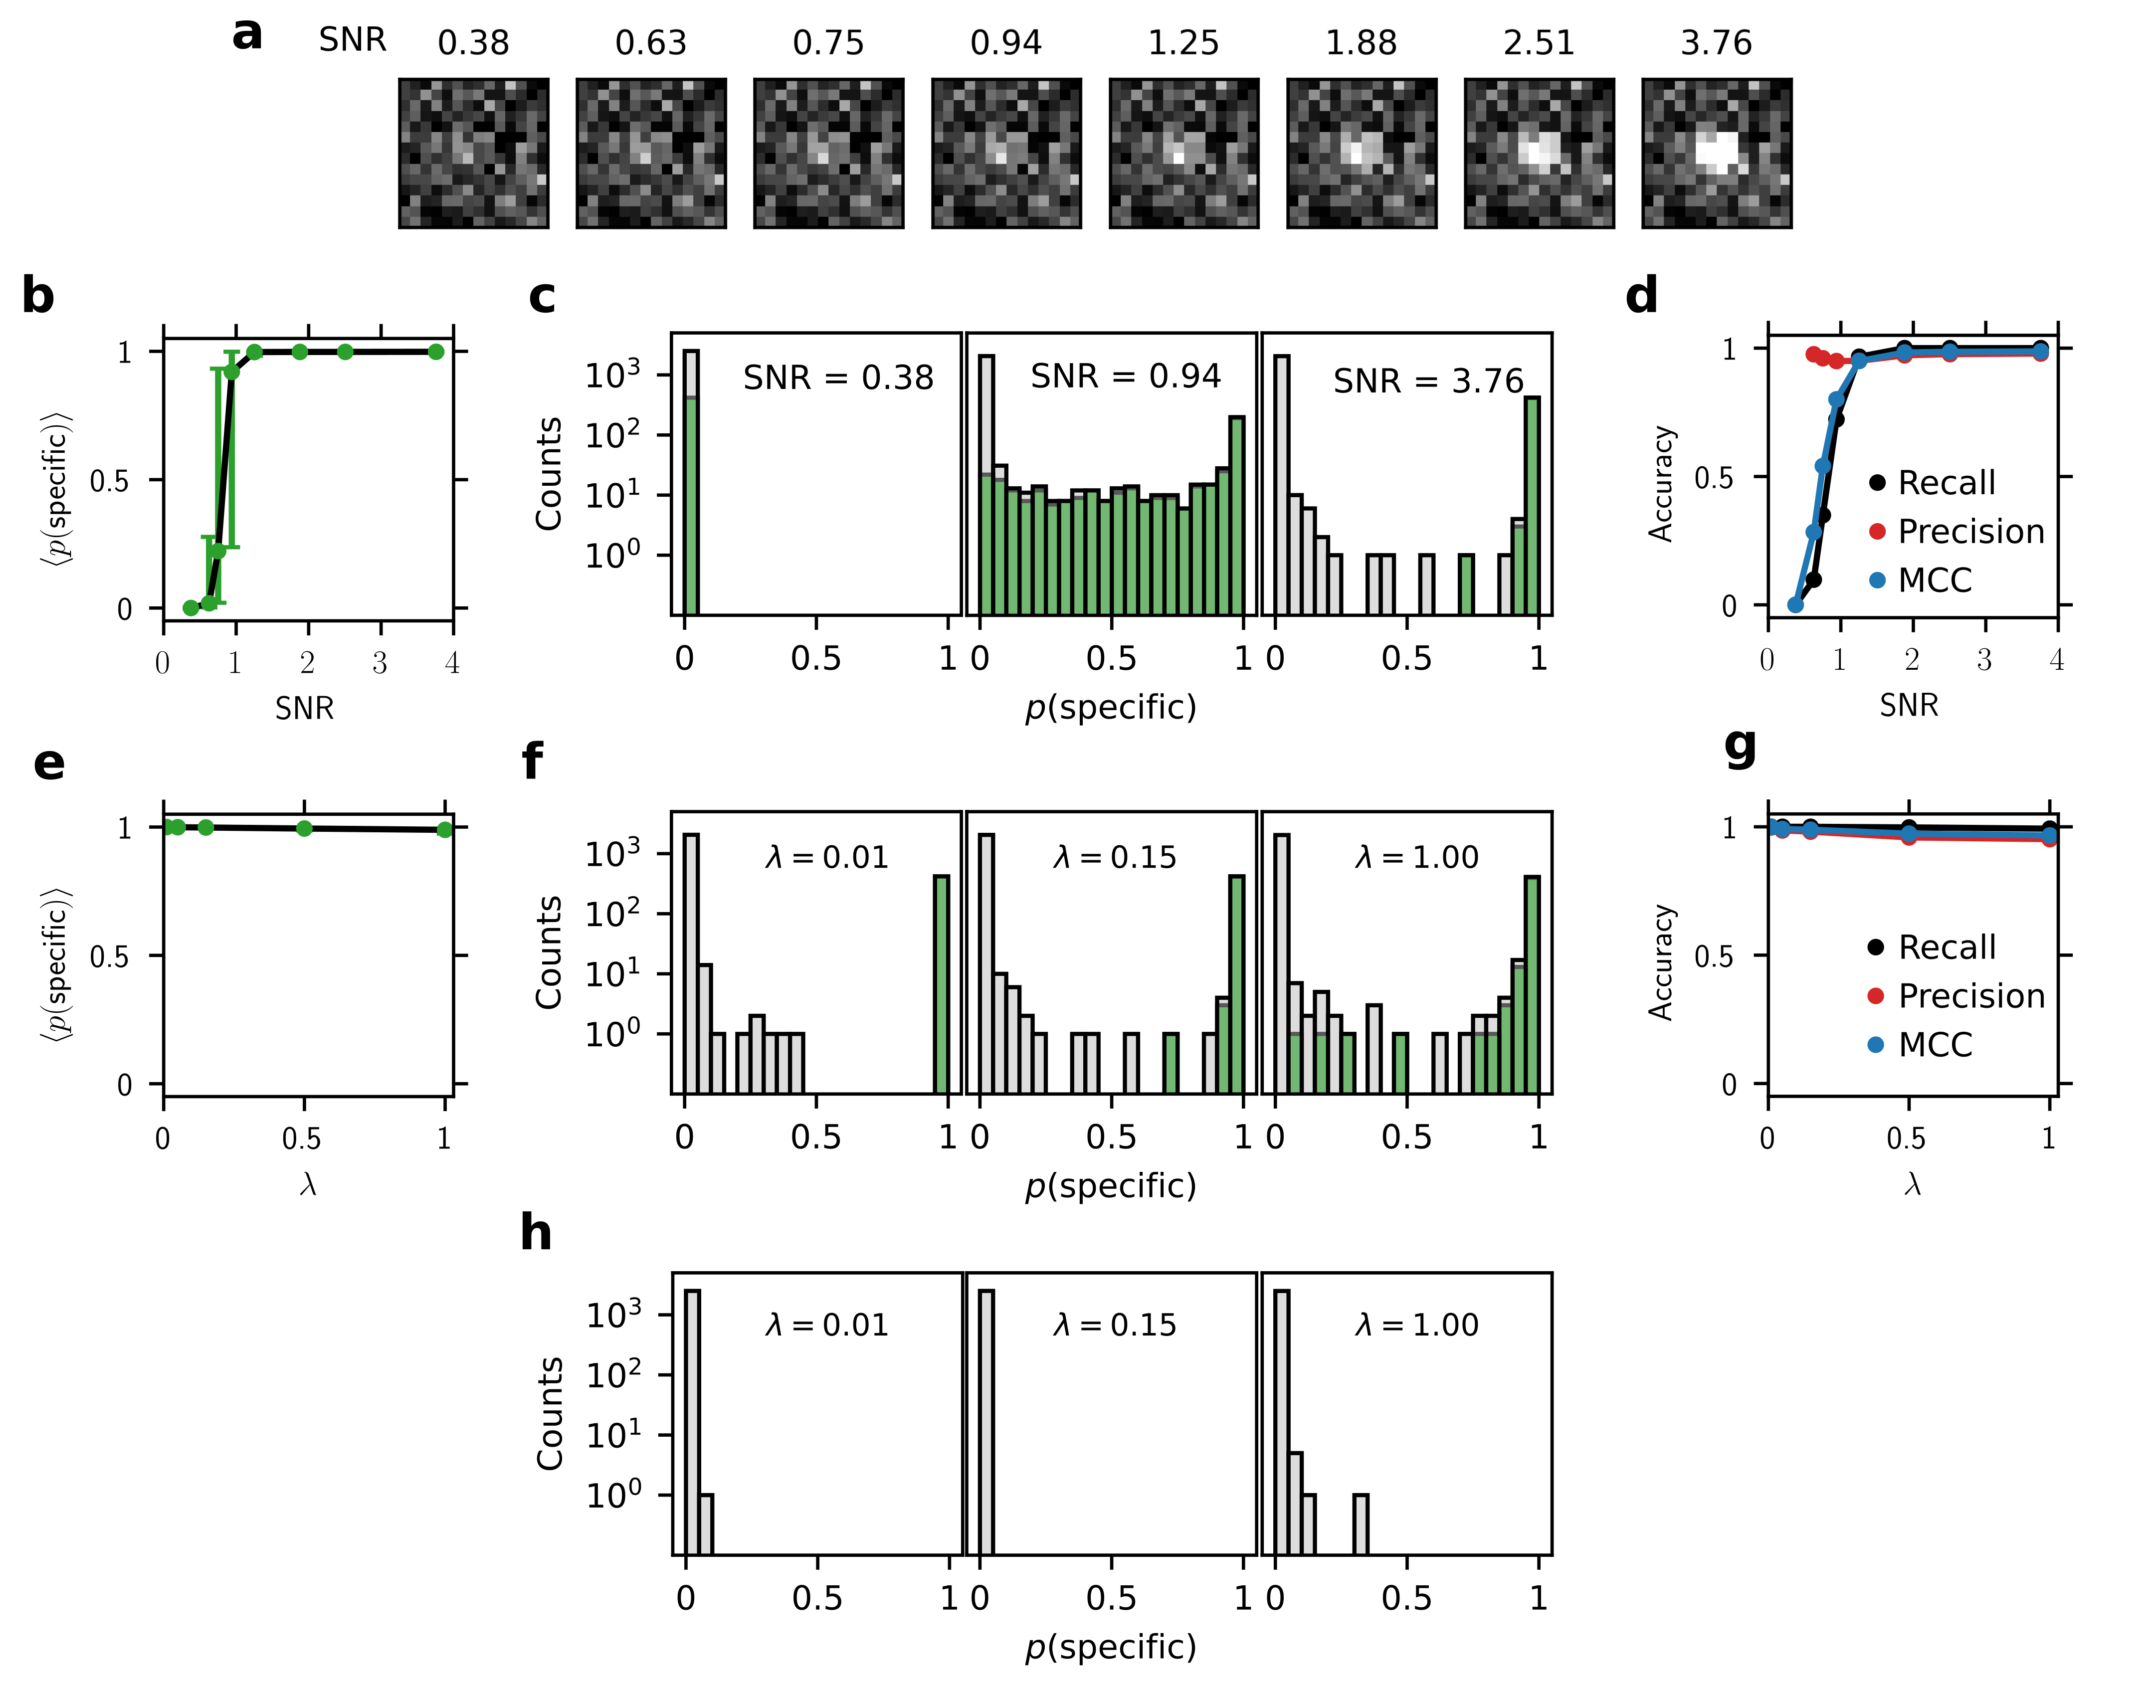
\includegraphics[width=\linewidth]{figures/figure5/figure5.png}
\caption{Performance comparison of the Bayesian method with the heuristic spot thresholding algorithm on real experimental data.}
\label{fig:real_data}
\end{figure}

\begin{figure}
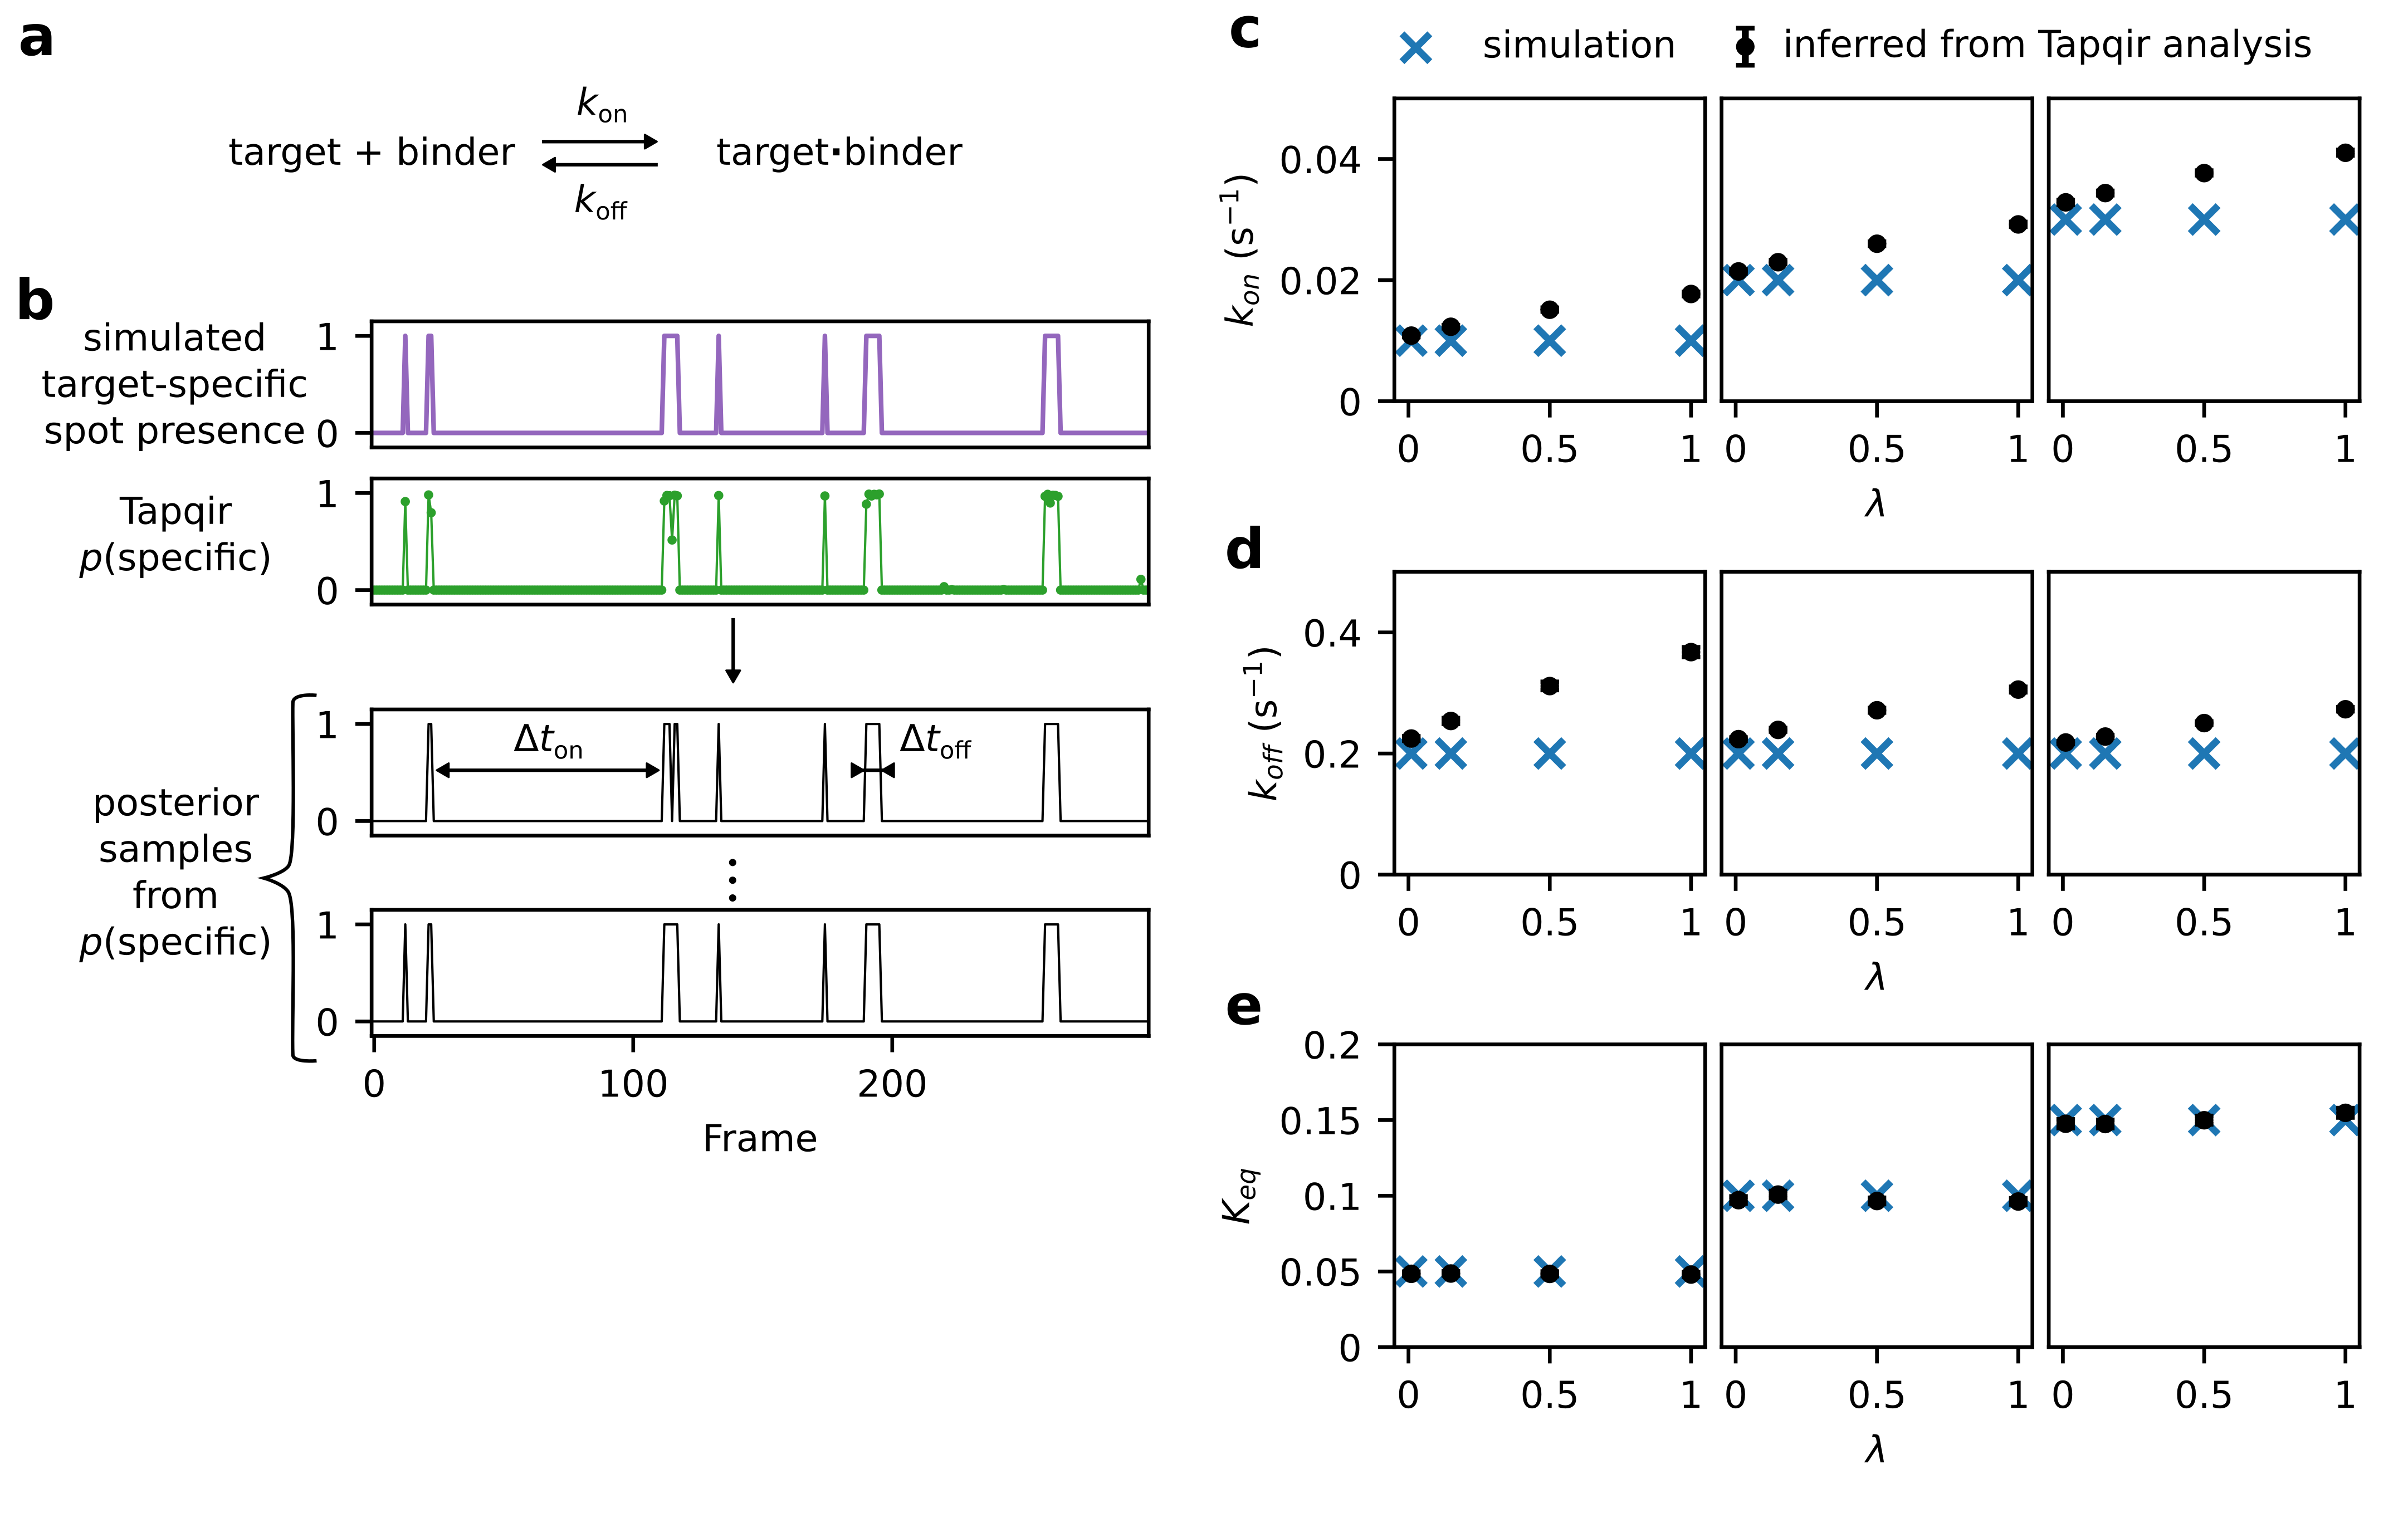
\includegraphics[width=\linewidth]{figures/figure6/figure6.png}
\caption{Performance comparison of the Bayesian method with the heuristic spot thresholding algorithm on real experimental data.}
\label{fig:real_data}
\end{figure}

\begin{figure}
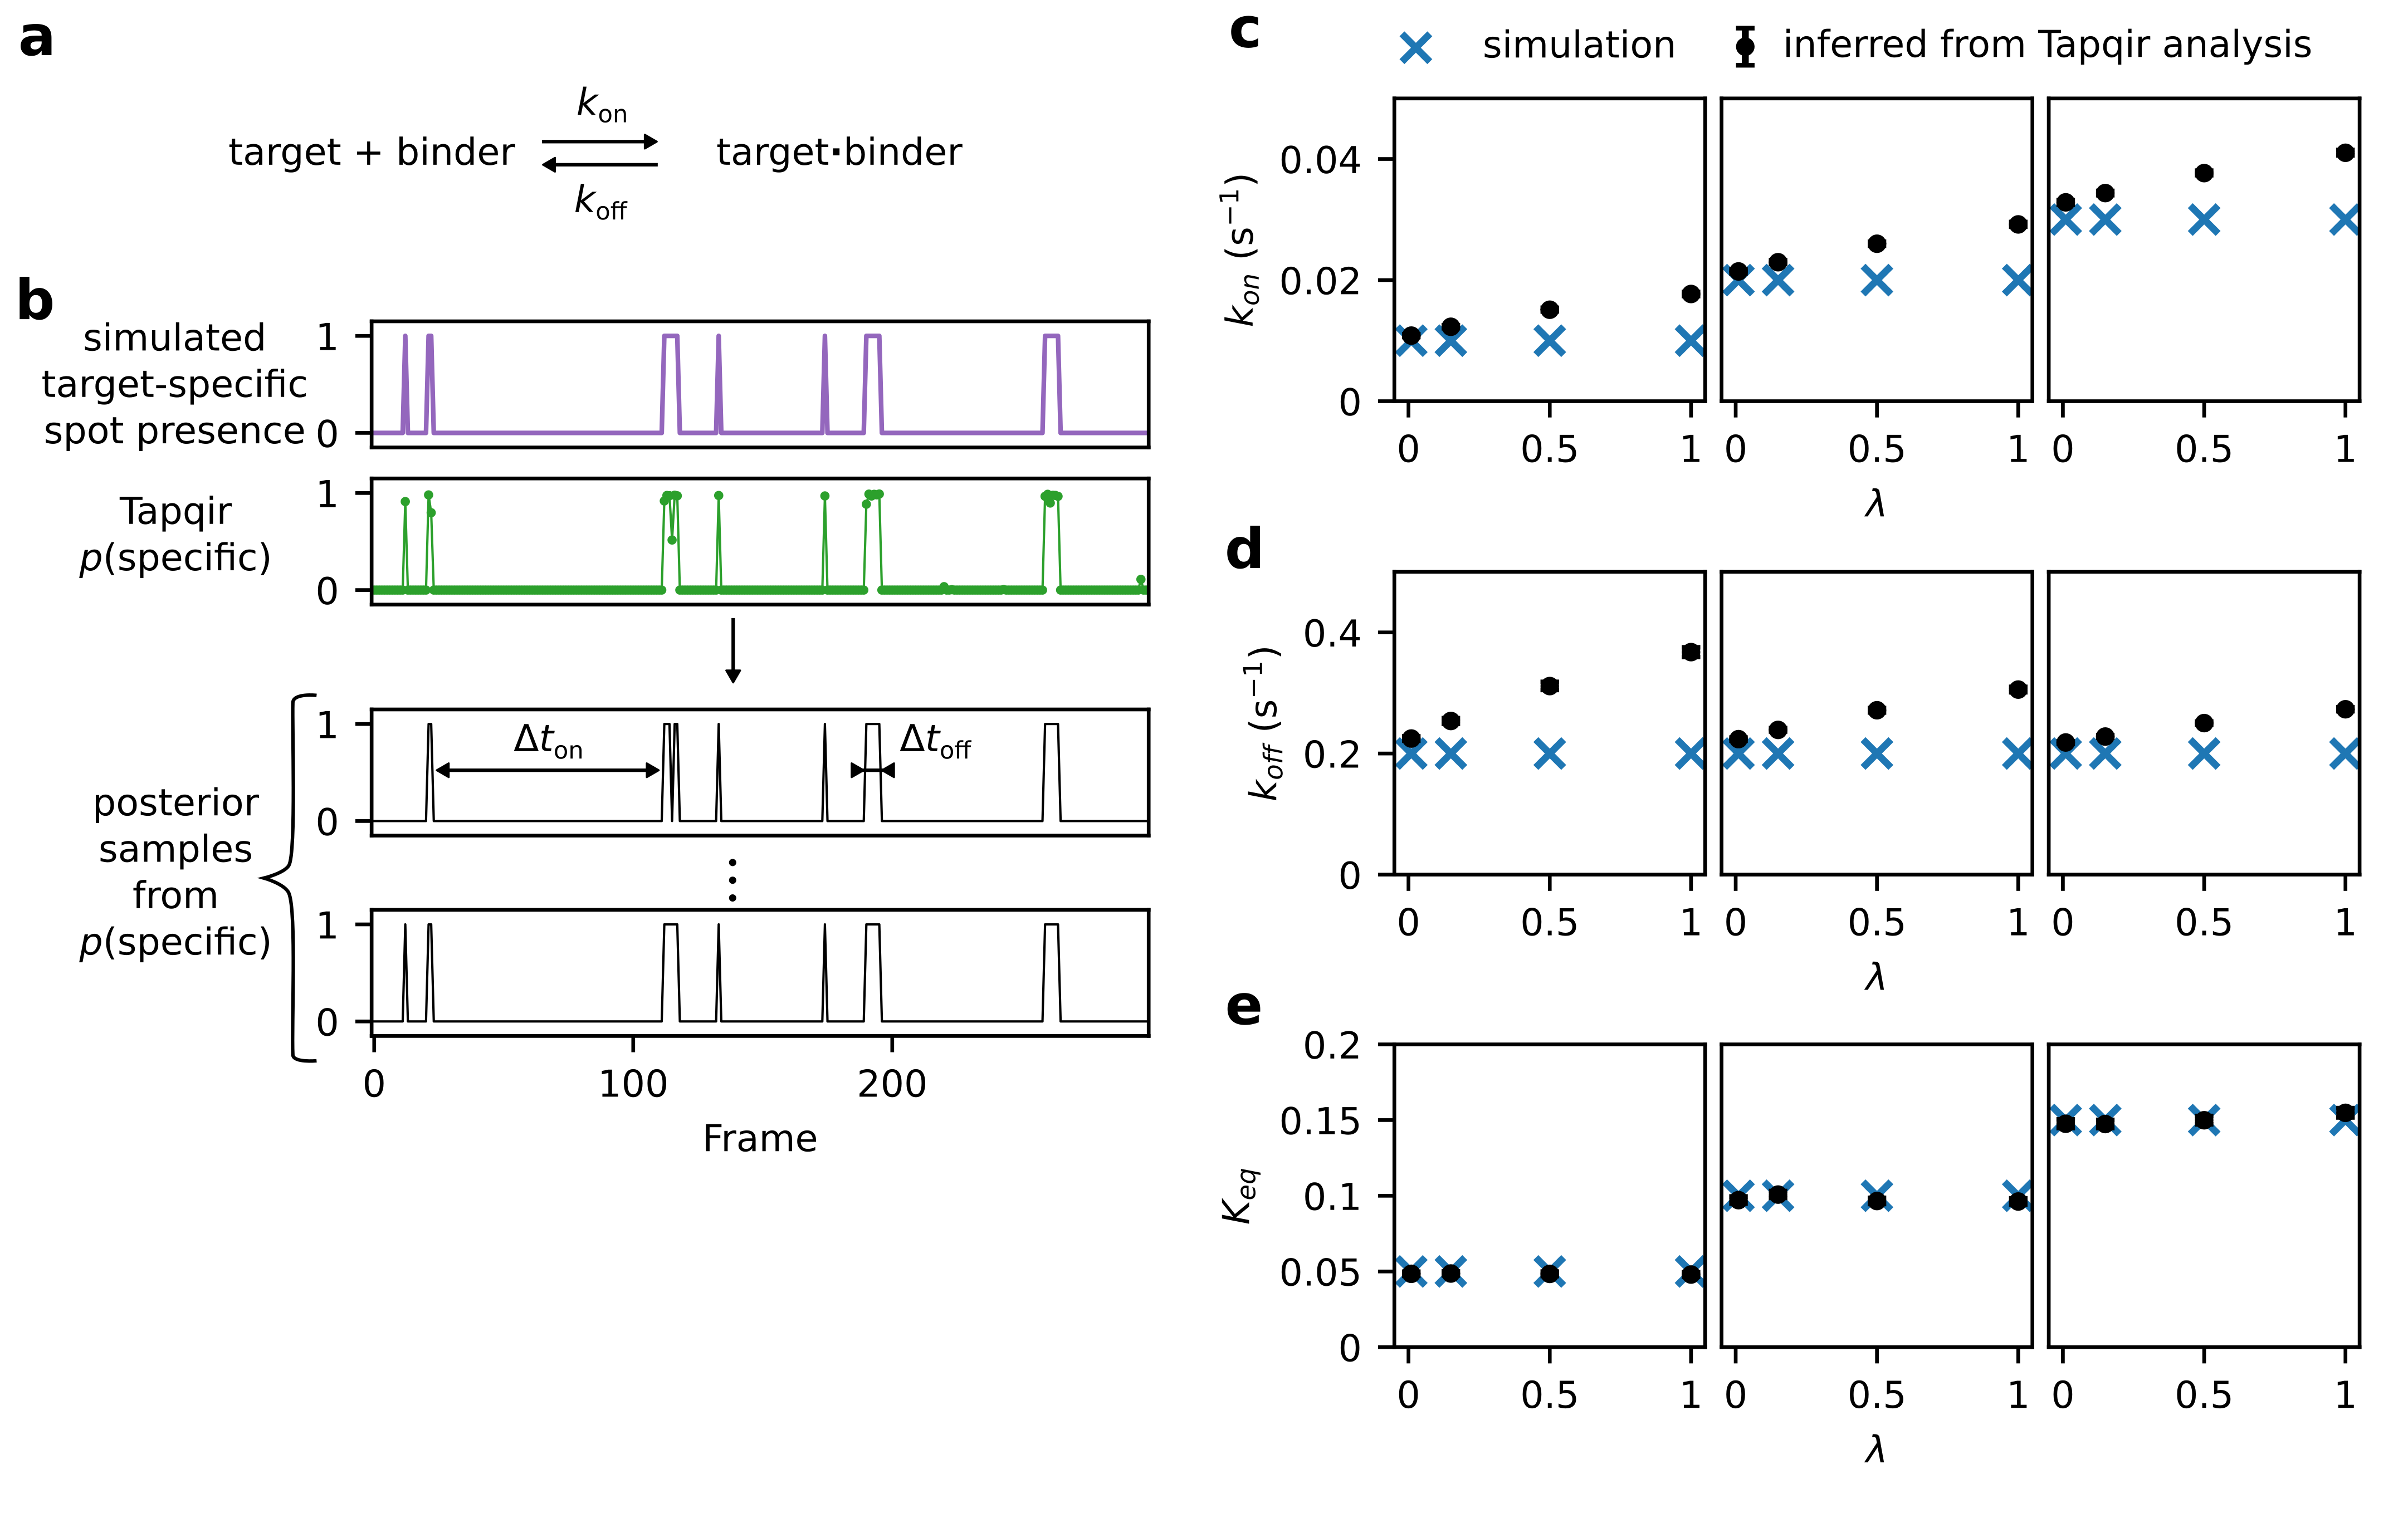
\includegraphics[width=\linewidth]{figures/figure6/figure6.png}
\caption{Performance comparison of the Bayesian method with the heuristic spot thresholding algorithm on real experimental data.}
\label{fig:real_data}
\end{figure}

\subsubsection{Simulated data}

In a second comparison, a series of simulated data sets were constructed for a range of signal-to-noise values. For each S/N, a set of 7,500 images (15 AoIs, 500 frames) of 14 by 14 pixels shape were generated using our probabilistic generative model. Each image is a combination of the background intensity plus randomly sampled 2-D Gaussian spots bound at the target and off-target with the intensity noise generated according to Gamma distribution.

Comparison of two methods showed similar performance on simulated data (Figure \ref{fig:simulated_data}). Taken together, these data demonstrated that the Bayesian method performs as well as or even better than the best existing CoSMoS data analysis method. Furthermore, Bayesian method achieves this performance automatically, with no adjustable parameters whatsoever, unlike the heuristic spot picker which attains this level of performance only after careful subjective trial-and-error manual adjustment of its three threshold parameters, a process that must be repeated tediously for each data set analyzed. Finally, our new Bayesian method produces a spot probability estimate for each image (not merely a Boolean spot/no spot determination) that can be used to inform subsequent kinetics calculations based on the results (e.g., the HMM analysis).

%\begin{figure}
%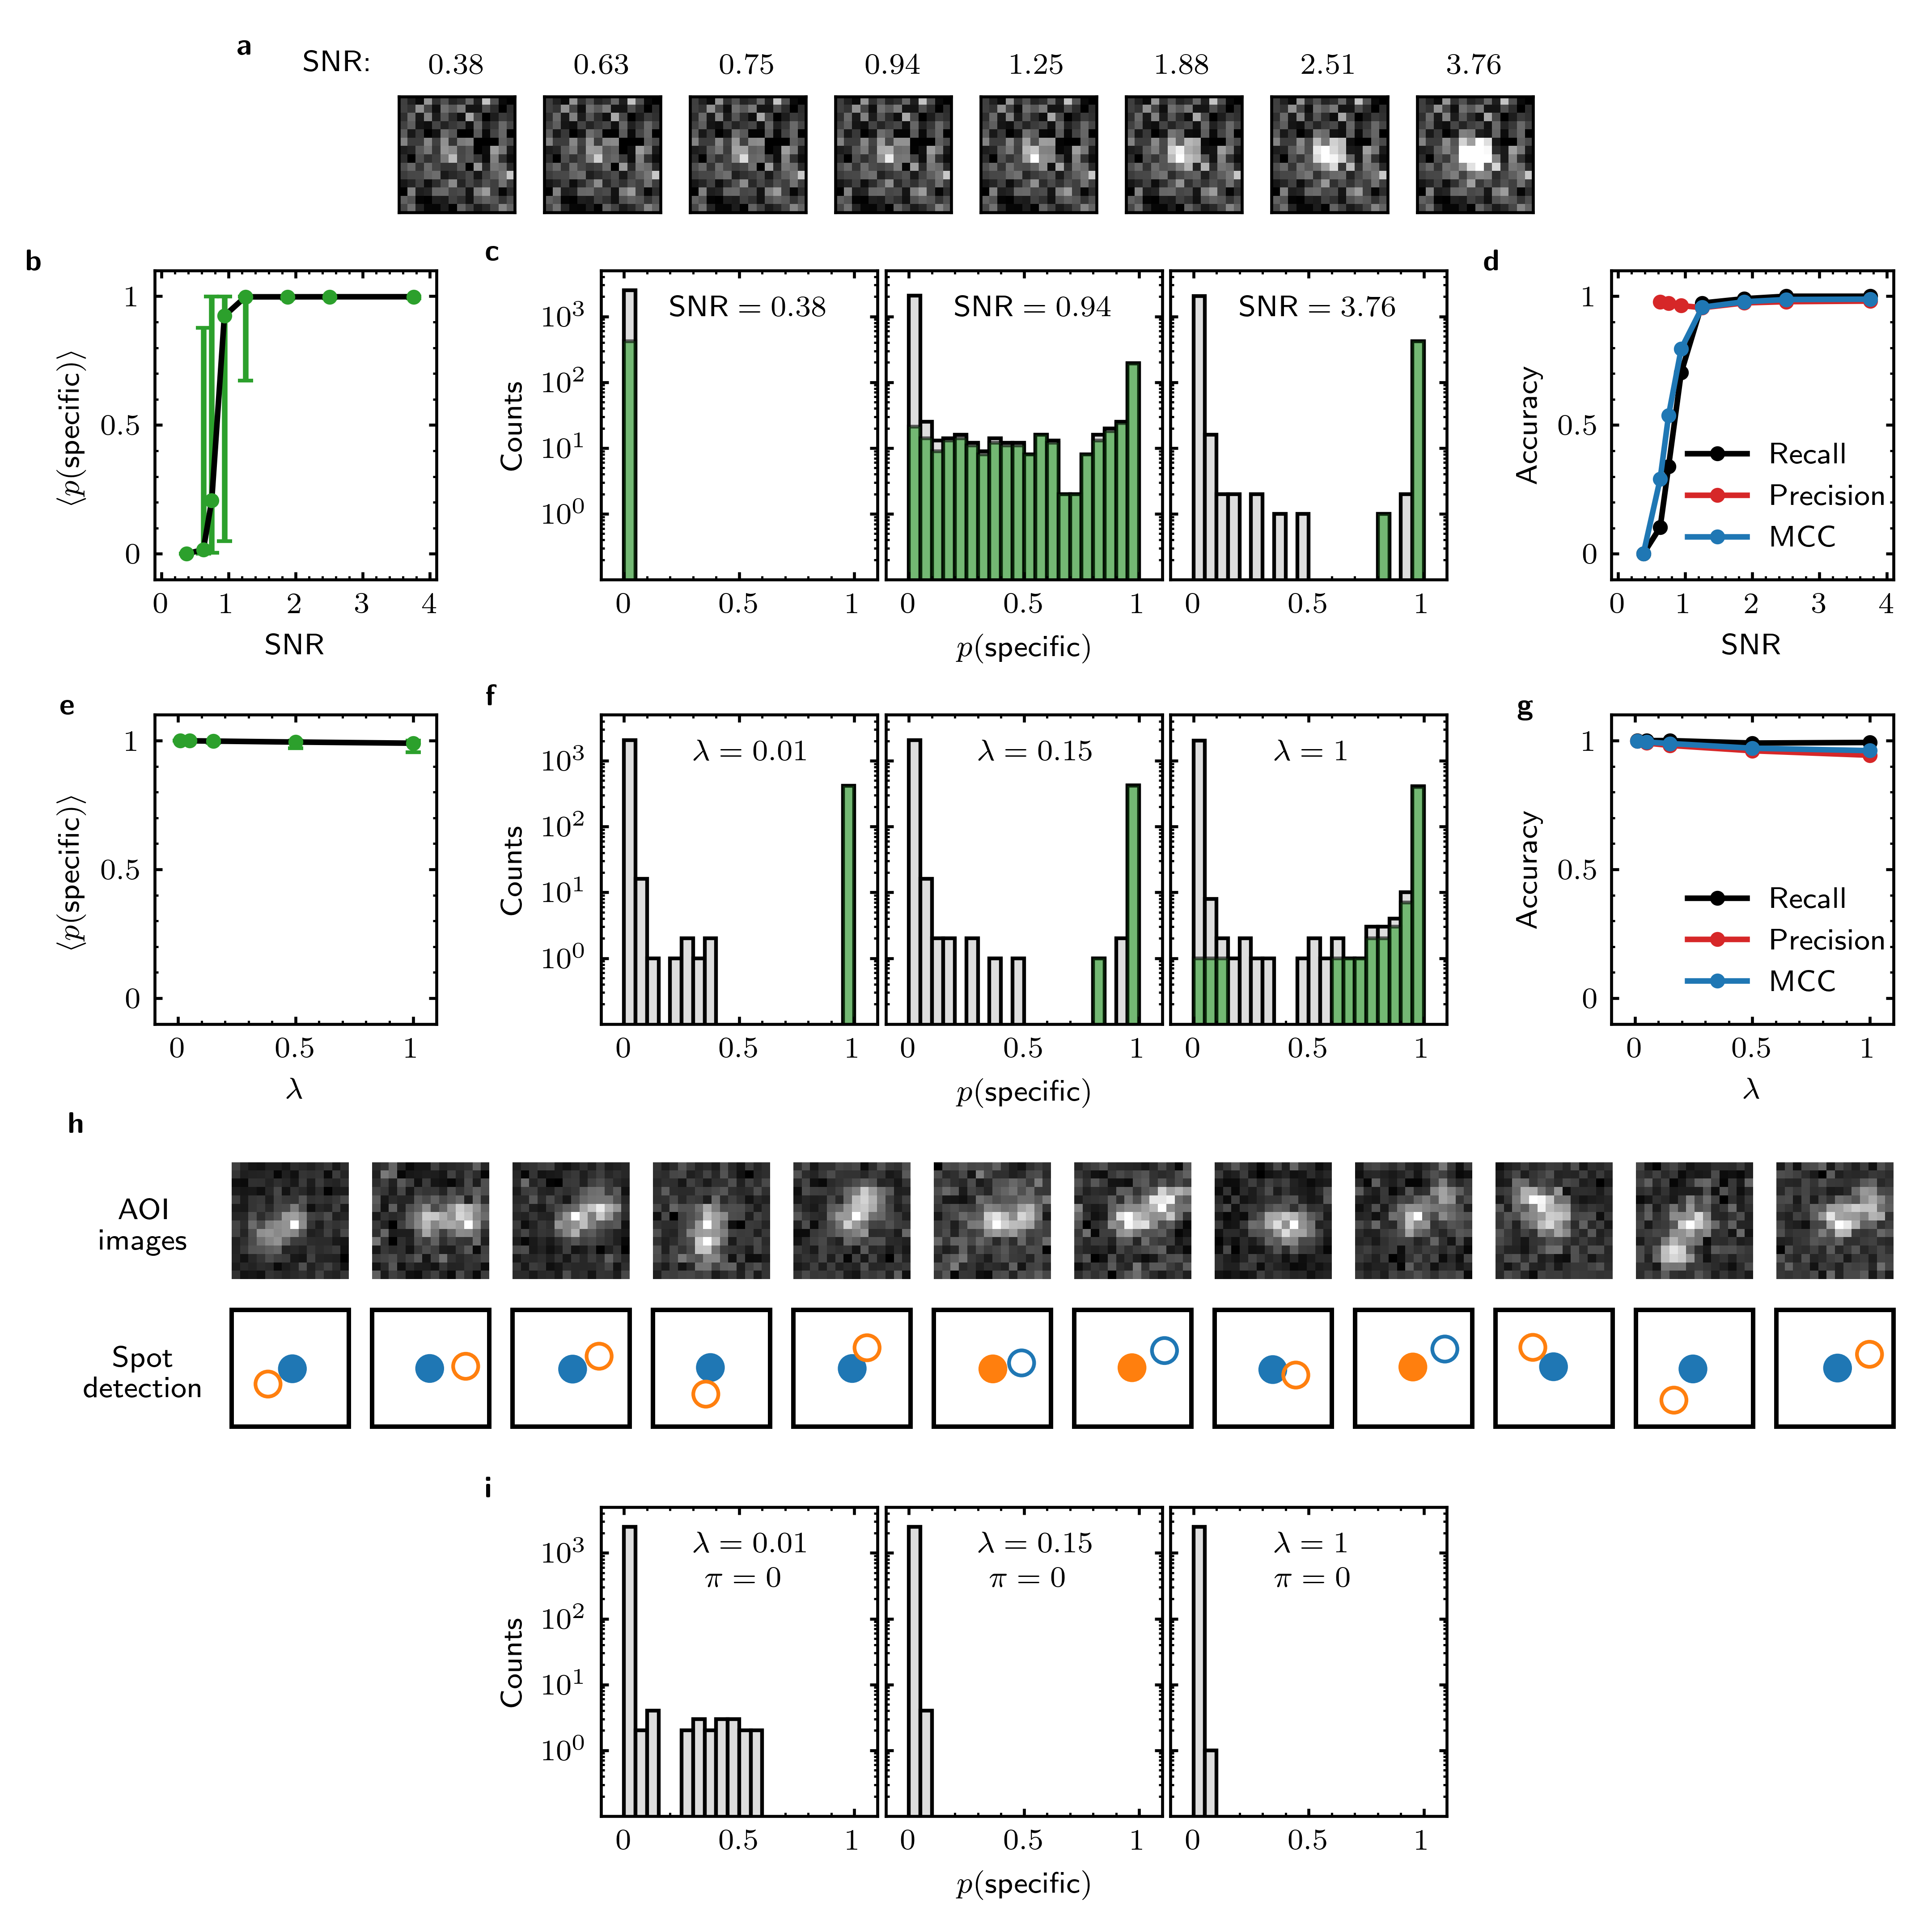
\includegraphics[width=\linewidth]{figures/figure5.png}
%\caption{Performance comparison of the Bayesian method with the heuristic spot thresholding algorithm on simulated data.}
%\label{fig:simulated_data}
%\end{figure}